\documentclass[11pt,twocolumn]{report}
\usepackage{graphicx}
\usepackage{a4wide}
\usepackage[english]{babel}
\usepackage{amsfonts}
\usepackage{amsthm}
\usepackage{amsmath}
\graphicspath{ {images/} }

\author{He Chen, Henri Maxime Demoulin, Gabrielle De Micheli}
\title{CIS520 Final Project Report}

\begin{document}
\maketitle
\section*{Introduction}
    In this report we detail our pre-processing steps, as well as four methods we analyzed during the project. We then proceed to an in depth analysis of the methods, and also present a visualization of the data which was instrumental in gaining accuracy.

\section*{Methods Accuracy Report}
    % Results for each method you tried (try to use checkpoints to get test set accuracy for each of your methods)
    First, let us explain the preprocessing steps that we have taken, in order to purify the features from low value words. We did delete all the English, French, and Spanish common stop words \ref{stopwords}, words containing only one character, unicode words, words such as ``http'' and ``rt'', and a bunch of symbols not bearing emotions, such as ``-->'' or ``\_\_''. We tested multiple combinations of features removals, and observed that trimming too many "non emotional symbols", such as the ones we mentionned before, was not beneficial in terms of cross-validation error, nor in testing error on the leaderboard. We suppose that this is due to the correlation between such symbols and the other words in the text.
    \par
	Another thing that we have done, in order to check for words worth deletion, was to iterate through all $10,000$ of the word columns, and if deleting a column yielded significantly better cross validation accuracy ($1.5$ percent or better), then we deleted that column in the preprocessing step. However, the results where not as good as expected, and we ended up with a higher cross-validation error ($2$-$3$ percents) than we started with.
    
    \subsection*{Generative Methods}
    \subsubsection{Naive Bayes}
    We start by using Naive Bayes only on the words. This method gave us around $80 \%$ testing accuracy on the leaderboard, without pre-processing. Adding a combination of the pre-processing described above, the testing accuracy raised to $81.42\%$. In order for Naive Bayes to work, we got rid of all the words that do not appear in any tweets, since $fitncb()$ assume conditional independence and does not handle words of probability $0$. We use a variation of the bag of word model, where the word counts is set to 1 if a word appears in a tweet and zero otherwise.
    \par
    We have also tried and tested $\log(w_i + 1)$ and $\sqrt(w)$, but doing that made the accuracy of Naive Bayes go bad $(22-35)$ percent of cross-validation error. So we concluded that the best way was simply checking if the word exists or doesn't exist (0 or 1). From our experience, Naive Bayes is both extremely accurate and extremely fast when used on the word counts.   
   
    
    \subsection*{Discriminative Methods}
    \subsubsection{Linear Regression}
	We primarily did Linear Regression on the CNN features only. We tried it on the raw CNN features, the CNN features max pooled to various degrees, and the CNN features mean pooled to various degrees. At first we tried Elastic Net regression, which got around $65$ percent cross-validation accuracy, give or take $3$ percent for all of the different pooling methods. Then we tried $L1$ regression, which got pretty identical results as Elastic Net. Then we tried $L2$ regression which was slightly better than Elastic Net and $L1$, with about $68$ percent cross-validation accuracy. 
    \par
    In all 3 of these regression methods, we were not able to get much better than $68$ percent cross-validation accuracy, which combined with the bag of words Naive Bayes, resulted in a $78-80$ percent cross-validation accuracy. Our conclusion was that linear regression was not appropriate for the CNN features, and so we did not incorporate it in our leaderboard model. 
    
     \subsubsection{Random Forest}
     We tried random forest on the words only but we observed the following: with $20$ trees, cross-validation error was $0.2167$, while with $100$ trees it was $0.2116$. Cross-validation error stayed stable with $500$ and $1000$ trees, which is consistent with previous reports of random forest accuracy, where the model tends to overfit past the hundreds trees, without yielding much gain in accuracy \ref{latinne2001limiting,oshiro2012many}. We note that we used the same pre-processing steps we took with Naive Bayes.

    \subsubsection{SVM}
    Using SVM with an RBF (Radial Basis Function) kernel function, results in a cross-validation error of $0.3813$. With a linear kernel, the cross validation error is $0.26$. However, we note that using RBF with the full wordcount (in lieu of the binary presence/absence indicator), we have a cross validation error of $0.3776$. Using the linear kernel with the full wordcount yields a cross-validation error of $0.2626$.
    
    \subsection*{Instance based Methods}
    \subsubsection{KNN}
    
    We use KNN on all four datasets and get a cross-validation error of $0.3556$.
   
    \subsection*{Semi-supervised methods}
    \subsubsection*{PCA}
    We used PCA on both \textit{image dataset} and \textit{word dataset}. On the words, PCA with all the PCs combined with SVM gives a cross-validation error of 0.0324. We do the same again but only with 1000 PCs. This gives an error of 0.1198. Moreover, using 570 PCs (corresponding to 50MB), we get a cross validation error of 0.1509.\\
    
    
   On the \textit{word dataset}, we also try using PCA with various numbers of PCs (all, 500 ...) and this time, combined with random forest. This gives a cross validation error of 0.0064. The test-accuracy is 0.7491.\\
    
    

\section *{Methods Analysis}
    % Analysis of your experiments. What worked and what didn’t work? Why not? What did you do to try to fix it? Simply saying “I tried XX and it didn’t work” is not enough.

    We tried SVM only on words, and notice that it performs better than KNN.

\section*{Visualization}
    % An interesting visualization of one of your models. For instance, find the words that most correlate with the outcome.
    In order to get a better sense of what words where most impactful during our classification, we consider the well-classified ones and use their count to create the word cloud bellow:
    
    \begin{center}
    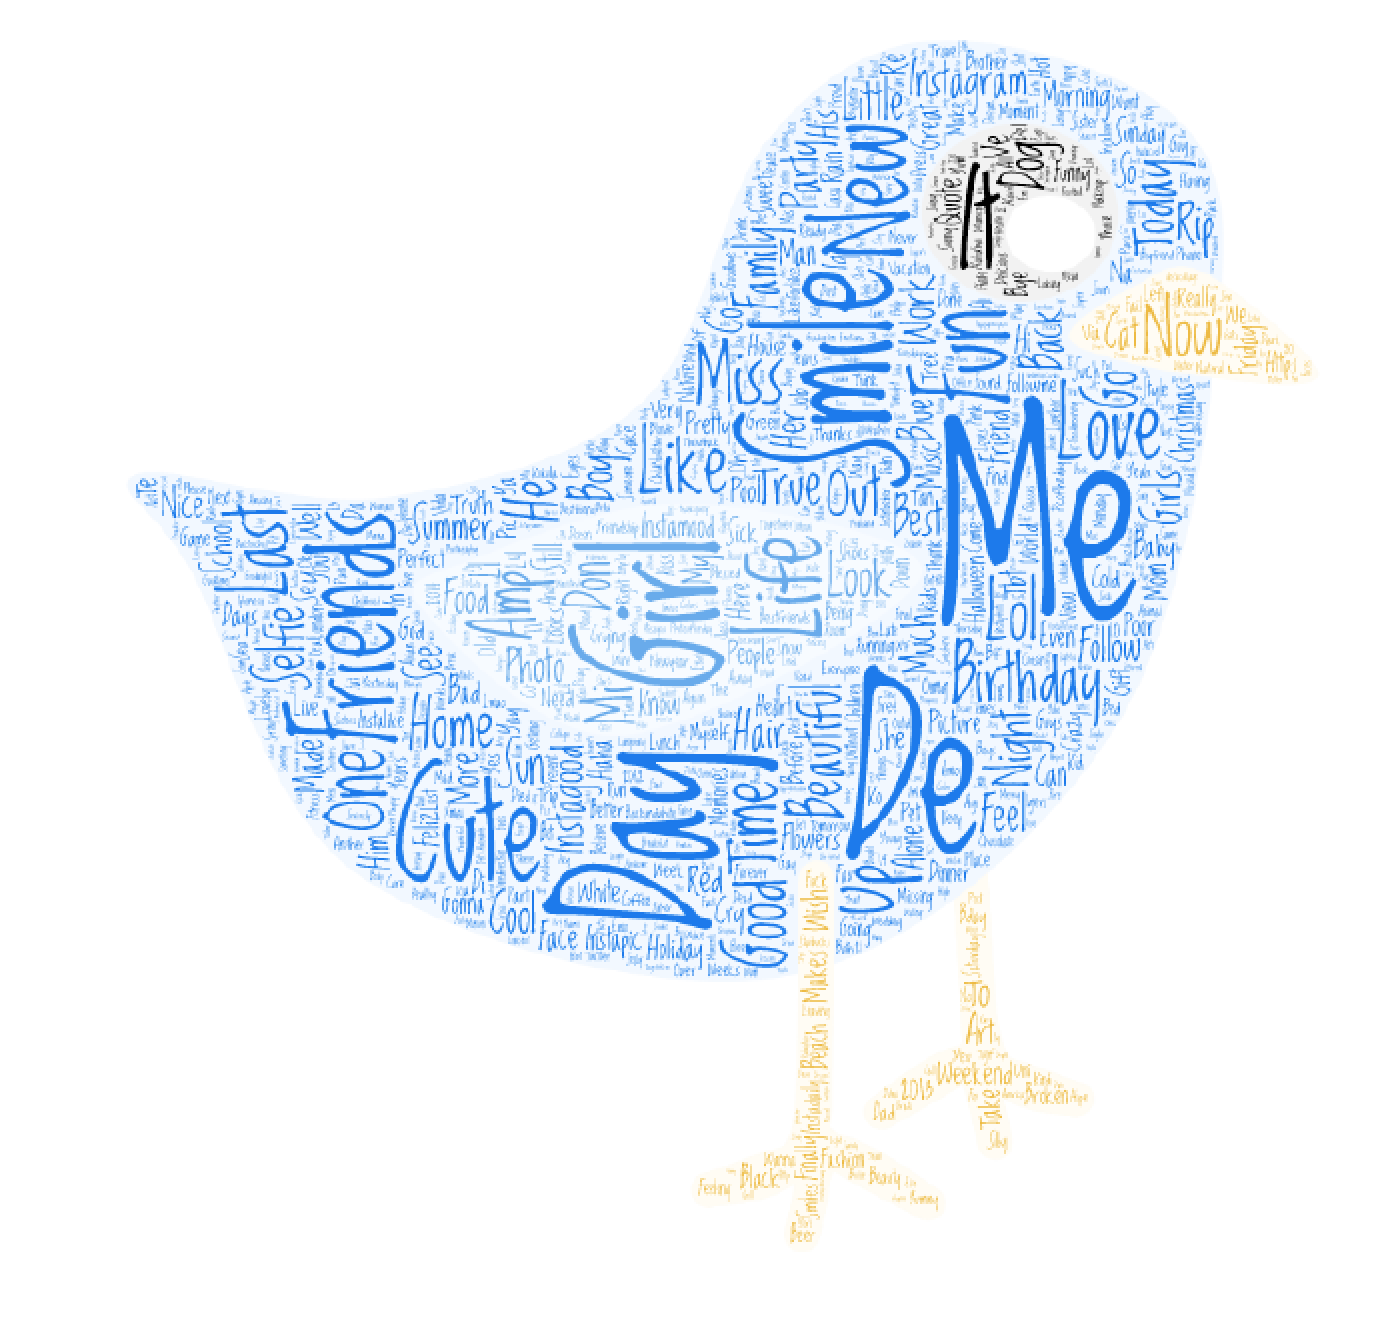
\includegraphics[scale=0.45]{cloud}
    \end{center}

    \bibliographystyle{abbrv}
    \bibliography{report}

\end{document}
